\documentclass[12pt]{article}
\usepackage[utf8]{inputenc}
\usepackage{enumerate}
\usepackage{geometry}                % See geometry.pdf to learn the layout options. There are lots.
\geometry{letterpaper}                   % ... or a4paper or a5paper or ... 
%\geometry{landscape}                % Activate for for rotated page geometry
\usepackage[parfill]{parskip}    % Activate to begin paragraphs with an empty line rather than an indent
\usepackage{graphicx}
\usepackage{amssymb}
\usepackage{amsmath}
\usepackage{epstopdf}
\usepackage{comment}
\usepackage{alltt}
\usepackage{url}
\usepackage{xcolor}
\DeclareGraphicsRule{.tif}{png}{.png}{`convert #1 `dirname #1`/`basename #1 .tif`.png}
\newcommand{\NB}[0]{\textcolor{red}{\textbf{!lähde!}}}
\newcommand{\TD}[0]{\textcolor{red}{\textbf{!TODO!}}}
\newcommand{\E}[0]{\textbf{Ebola }}

\title{EBORA - Evolutively Balanced Operational Rescue Algorithm}
\author{Team 41983}
\date{}                                           % Activate to display a given date or no date

\begin{document}

\setlength{\parindent}{0cm}

\section{Pictures}

\begin{figure}[h!]
	\begin{center}
		\makebox[\textwidth]{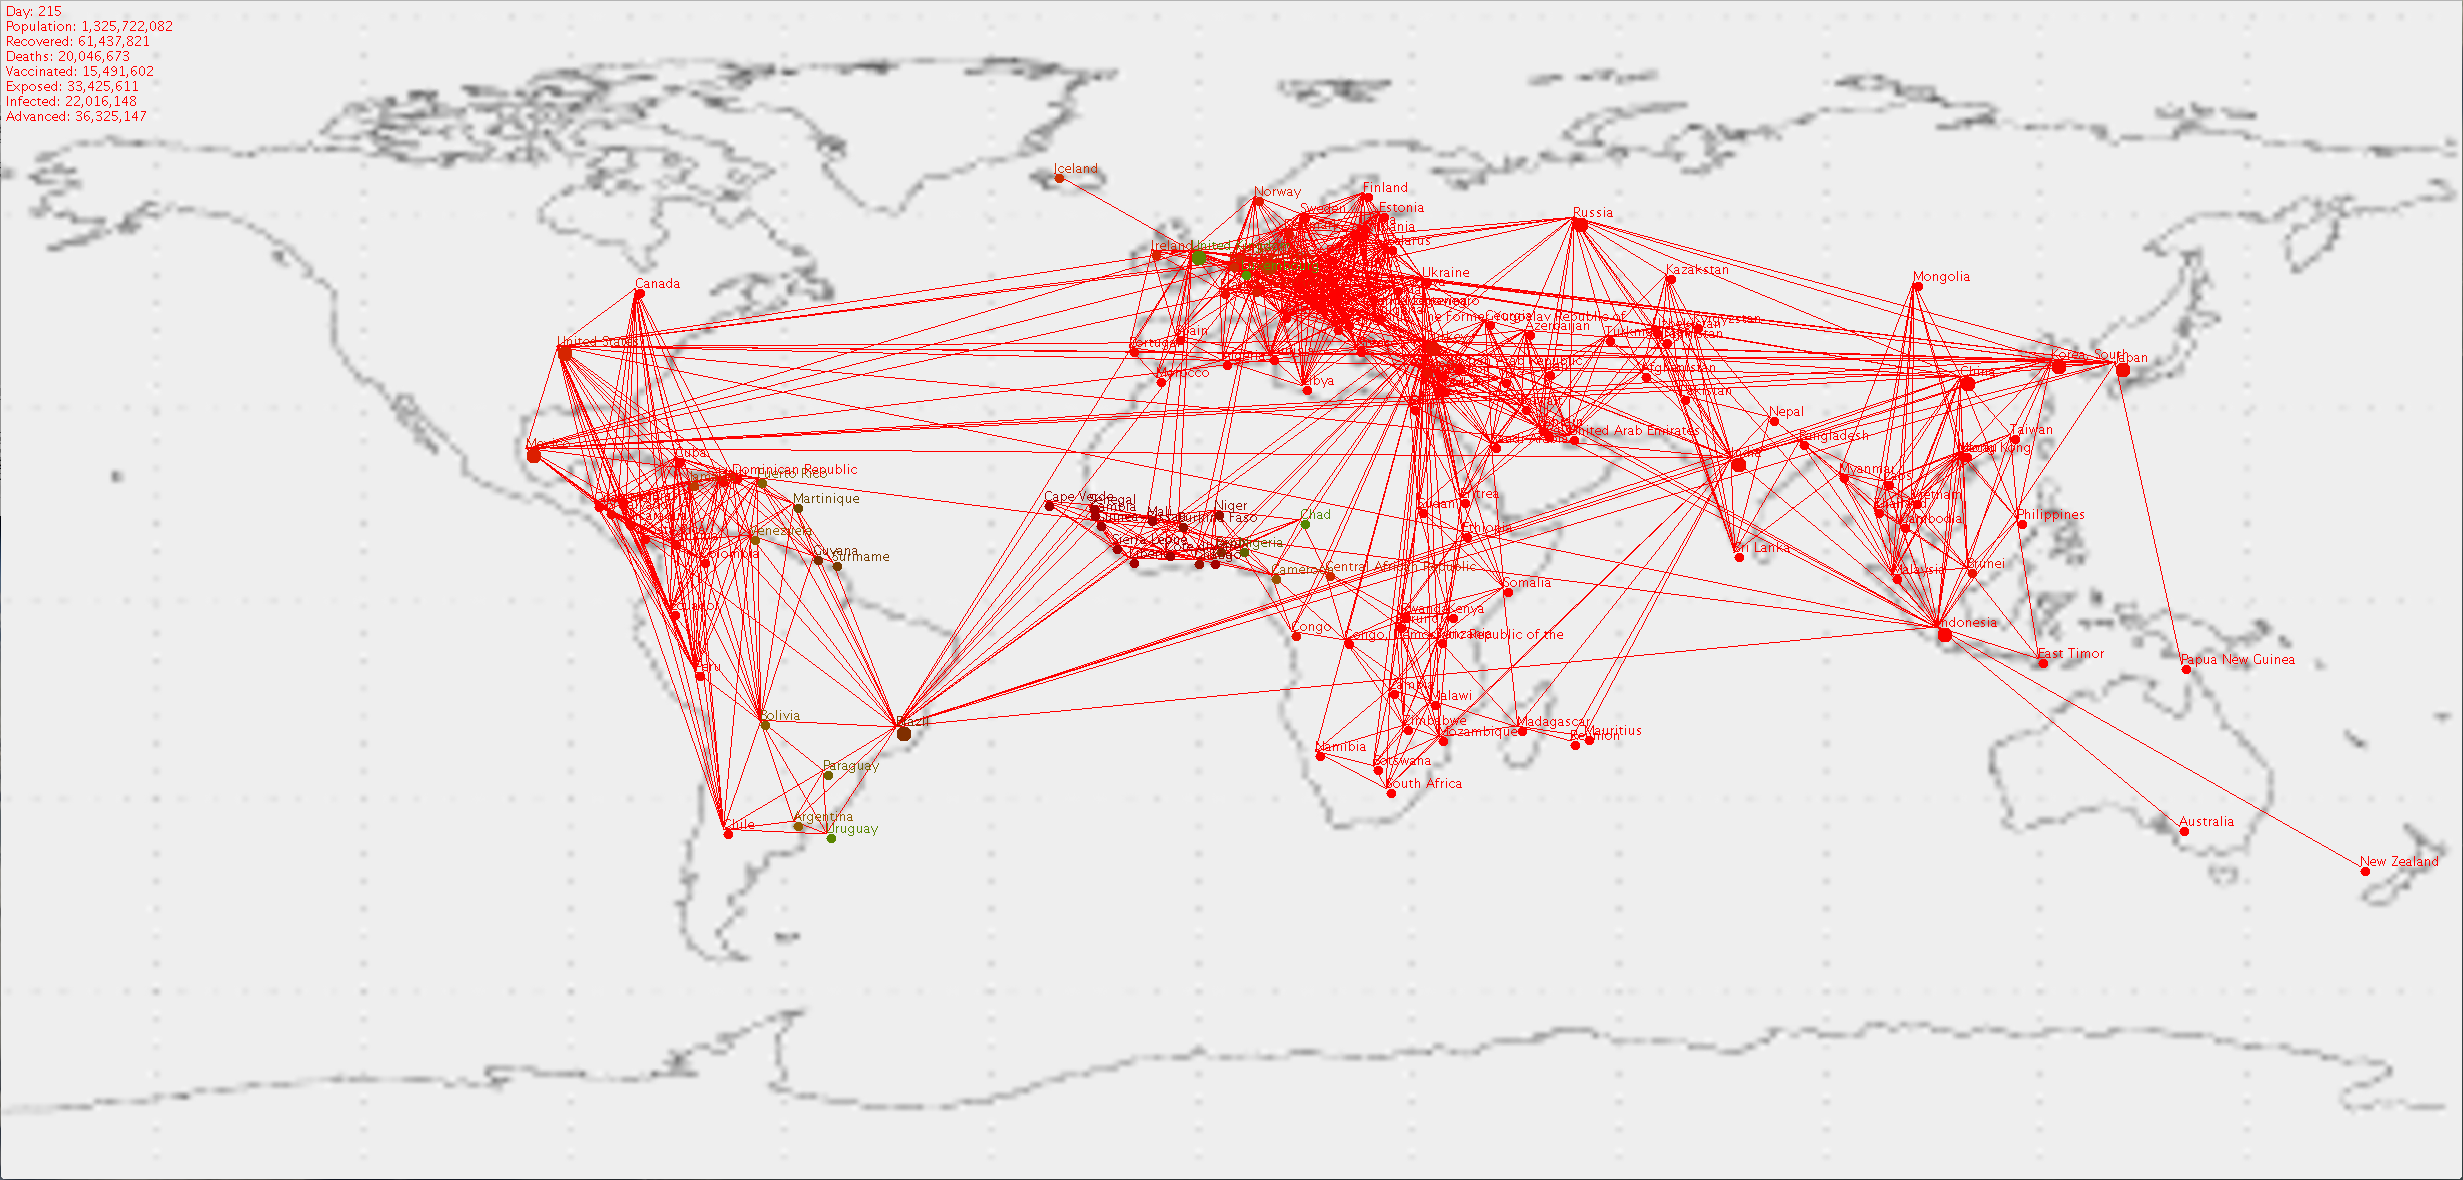
\includegraphics[width=500px]{map.png}}
	\end{center}
	\caption{A picture of a gull.}
\end{figure}

\begin{figure}[h!]
	\begin{center}
		\makebox[\textwidth]{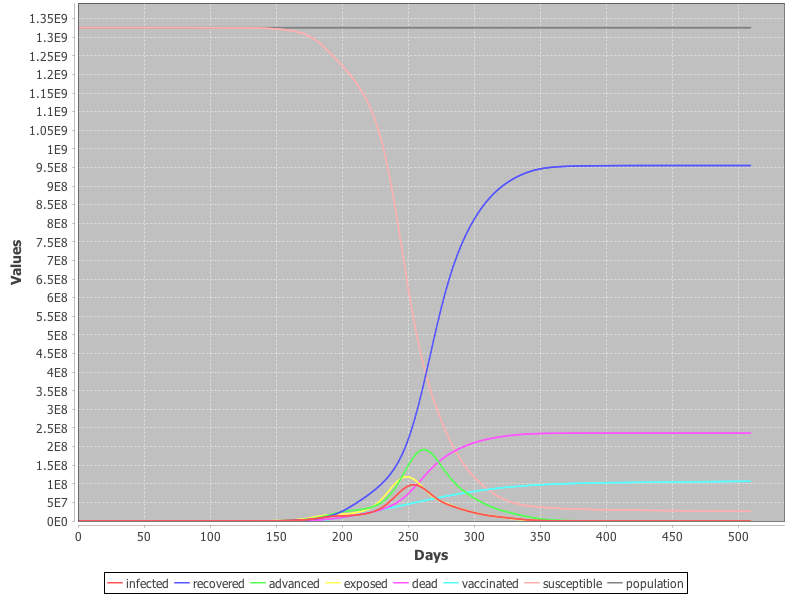
\includegraphics[width=500px]{chart.png}}
	\end{center}
	\caption{A picture of a gull.}
\end{figure}

\begin{figure}[h!]
	\begin{center}
		\makebox[\textwidth]{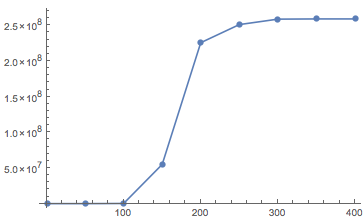
\includegraphics[width=500px]{Death.png}}
	\end{center}
	\caption{A picture of a gull.}
\end{figure}

\end{document}